\newcommand{\svcourse}{CST Part IA: Software Engineering and Security}
\newcommand{\svnumber}{1}
\newcommand{\svvenue}{Microsoft Teams}
\newcommand{\svdate}{2022-05-11}
\newcommand{\svtime}{15:00}
\newcommand{\svuploadkey}{CBd13xmL7PC1zqhNIoLdTiYUBnxZhzRAtJxv/ytRdM1r7qIfwMsxeVwM/pPcIo8l}

\newcommand{\svrname}{Dr Sam Ainsworth}
\newcommand{\jkfside}{oneside}
\newcommand{\jkfhanded}{yes}

\newcommand{\studentname}{Harry Langford}
\newcommand{\studentemail}{hjel2@cam.ac.uk}


\documentclass[10pt,\jkfside,a4paper]{article}

\usepackage{tikz}
\usetikzlibrary{positioning}
\usepackage{pythonhighlight}

% DO NOT add \usepackage commands here.  Place any custom commands
% into your SV work files.  Anything in the template directory is
% likely to be overwritten!

\usepackage{fancyhdr}

\usepackage{lastpage}       % ``n of m'' page numbering
\usepackage{lscape}         % Makes landscape easier

\usepackage{verbatim}       % Verbatim blocks
\usepackage{listings}       % Source code listings
\usepackage{graphicx}
\usepackage{float}
\usepackage{epsfig}         % Embed encapsulated postscript
\usepackage{array}          % Array environment
\usepackage{qrcode}         % QR codes
\usepackage{enumitem}       % Required by Tom Johnson's exam question header

\usepackage{hhline}         % Horizontal lines in tables
\usepackage{siunitx}        % Correct spacing of units
\usepackage{amsmath}        % American Mathematical Society
\usepackage{amssymb}        % Maths symbols
\usepackage{amsthm}         % Theorems

\usepackage{ifthen}         % Conditional processing in tex

\usepackage[top=3cm,
            bottom=3cm,
            inner=2cm,
            outer=5cm]{geometry}

% PDF metadata + URL formatting
\usepackage[
            pdfauthor={\studentname},
            pdftitle={\svcourse, SV \svnumber},
            pdfsubject={},
            pdfkeywords={9d2547b00aba40b58fa0378774f72ee6},
            pdfproducer={},
            pdfcreator={},
            hidelinks]{hyperref}

\renewcommand{\headrulewidth}{0.4pt}
\renewcommand{\footrulewidth}{0.4pt}
\fancyheadoffset[LO,LE,RO,RE]{0pt}
\fancyfootoffset[LO,LE,RO,RE]{0pt}
\pagestyle{fancy}
\fancyhead{}
\fancyhead[LO,RE]{{\bfseries \studentname}\\\studentemail}
\fancyhead[RO,LE]{{\bfseries \svcourse, SV~\svnumber}\\\svdate\ \svtime, \svvenue}
\fancyfoot{}
\fancyfoot[LO,RE]{For: \svrname}
\fancyfoot[RO,LE]{\today\hspace{1cm}\thepage\ / \pageref{LastPage}}
\fancyfoot[C]{\qrcode[height=0.8cm]{\svuploadkey}}
\setlength{\headheight}{22.55pt}


\ifthenelse{\equal{\jkfside}{oneside}}{

 \ifthenelse{\equal{\jkfhanded}{left}}{
  % 1. Left-handed marker, one-sided printing or e-marking, use oneside and...
  \evensidemargin=\oddsidemargin
  \oddsidemargin=73pt
  \setlength{\marginparwidth}{111pt}
  \setlength{\marginparsep}{-\marginparsep}
  \addtolength{\marginparsep}{-\textwidth}
  \addtolength{\marginparsep}{-\marginparwidth}
 }{
  % 2. Right-handed marker, one-sided printing or e-marking, use oneside.
  \setlength{\marginparwidth}{111pt}
 }

}{
 % 3. Alternating margins, two-sided printing, use twoside.
}


\setlength{\parindent}{0em}
\addtolength{\parskip}{1ex}

% Exam question headings, labels and sensible layout (courtesy of Tom Johnson)
\setlist{parsep=\parskip, listparindent=\parindent}
\newcommand{\examhead}[3]{\section{#1 Paper #2 Question #3}}
\newenvironment{examquestion}[3]{
\examhead{#1}{#2}{#3}\setlist[enumerate, 1]{label=(\alph*)}\setlist[enumerate, 2]{label=(\roman*)}
\marginpar{\href{https://www.cl.cam.ac.uk/teaching/exams/pastpapers/y#1p#2q#3.pdf}{\qrcode{https://www.cl.cam.ac.uk/teaching/exams/pastpapers/y#1p#2q#3.pdf}}}
\marginpar{\footnotesize \href{https://www.cl.cam.ac.uk/teaching/exams/pastpapers/y#1p#2q#3.pdf}{https://www.cl.cam.ac.uk/\\teaching/exams/pastpapers/\\y#1p#2q#3.pdf}}
}{}


\begin{document}

\begin{enumerate}

\item From the Ethernet-attached machine with IP 10.11.6.1
(netmask 255.255.255.0), you use the command-line tool ``ping'' with
argument 10.11.7.1. Supposing all caches are initially empty, list the work
performed by each layer of the OSI stack, and the messages send up to the
point where ``ping'' reports the first round-trip time.

Let the sender be $A$, the router on the same LAN as $A$ be $R_A$, the
destination address be $B$ and the router on the same network as $B$ be $R_B$.

Ping uses ICMP -- which runs on top of IP\@. The method is ``send a
normal IP packet'' with a payload corresponding to an ICMP packet. ICMP
packets have the following form:
\begin{center}
\begin{tikzpicture}
\draw (0, 0) rectangle (2, 1) rectangle (4, 0) rectangle (6, 1);
\node at (1, 0.5) {Type};
\node at (3, 0.5) {Code};
\node at (5, 0.5) {Data};
\end{tikzpicture}
\end{center}
Type indicates what type of ICMP message is being sent. This is 8 for ICMP
echo (what Ping uses) and 0 for Echo reply (the response sent). Code is
always zero. Data contains the first 8 bytes of the packet which caused the
error -- in the case of ping the premise is false so Data is empty.
However, in general ICMP packets are sent after errors.

The stages are:

\begin{itemize}

\item $A$ constructs the ICMP packet as described, with Type=8 and all
other fields zero.

\item Next, $A$ must send the IP packet to $B$.

\item $A$ applies the netmask to the IP address of $B$ and determines $B$
is on a different LAN\@.

\item $A$ \textit{must} know its routers IP address (since it has an IP
address). But it may not know its routers MAC address.

\item So it uses ARP to find its routers MAC address

\item $A$ then builds the IP packet with the IP address corresponding to $B$
and wraps this in a frame with destination MAC address for $R_A$. The frame
is then sent to $R_A$.

\item $R_A$ receives $P$. After buffering, $R_A$ decrements the TTL -- if
it's zero, the packet is dropped. If nonzero the checksum is updated and
the process continues. looks up $IP(B)$ in the forwarding table and finds
no longest common prefix (since we assume no caches). So it initiates a
routing protocol (ie Distance Vector Routing). The results of the routing
protocol are stored in the Routing Table. This is then used to build a
Forwarding Table -- a mapping from routing prefix to port on which to
forward the packet.

\textbf{Does the router decrement the TTL before or after buffering the
packet?} Just a small thing I can't see mentioned anywhere. I'll assume
after.

\item $R_A$ then looks up the IP address for $B$, sends $P$ through the
switching fabric to the corresponding output port. This routing/forwarding
process is repeated at every router the packet encounters (although later
routers shouldn't have to do routing before forwarding).

\item Eventually the packet reaches router $R_B$.

\item $R_B$ performs ARP to find the address of $B$ and forwards the packet
onto $B$.

\item $B$ sees it's a ping and responds with an ICMP echo.

\item If the caches have been invalidated (or entries removed), the protocol
is the same in reverse. However, ideally $B$ would remember its routers MAC
address, $R_B$ would know the path to $R_A$ and $R_A$ would remember the
MAC address for $A$ -- meaning the return journey would just be a number of
lookups in forwarding tables.

\end{itemize}

ARP is implemented as follows:
\begin{itemize}

\item Each node keeps an ARP table which contains mappings from IP
addresses to MAC addresses. This table is invalidated intermittently since
IP addresses are not permanent.

\item The node broadcasts a request on the LAN for the mapping from IP
address to MAC address for node $n$.

\item Each node receiving the message looks up the IP address in its ARP
table. If there is an entry, it responds with the MAC address. If no entry is
found, it broadcasts the request to all nodes (except the node the message
came from).

\item We assume the use of spanning tree or some other protocol to prevent
forwarding loops.

\item Every node on the path to the destination node now has an entry in its
the forwarding table for the next node on the path. So the message can be
sent.

\end{itemize}

Distance Vector Routing:

A distance vector $D$ is a list of triples $(address prefixes, subnet mask,
distance, router)$ where $(a, s, d, r) \in D$ means that the subnet with
address prefix $a$ and subnet mask $s$ can be reached in distance $d$ by
forwarding to router $r$.

\begin{itemize}

\item Each router continuously sends its distance vector (except the
router to forward packets to) to its neighbours.

\item On receiving a distance vector, the router sets its own distance
vector to the elementwise minimum of the received distance vector (with the
distance field incremented) and distance vector received (breaking ties
deterministically by ID).

\item The forwarding table is then constructed by adding the in the
interface on which the packet should be sent to the distance vector.

\end{itemize}

\item What sequence of messages is required for a mobile device to lease an
IP address using DHCP? What characteristic of a network requires the use of
DHCP-Relay stations?

There are four messages required for a mobile device $A$ to lease an IP
address using DHCP\@. Firstly, mobile device $A$ broadcasts a message known
as a DHCP discover with source IP address $0.0.0.0$. The router hears this,
if it has available IP addresses, it will respond directly to the client
with a DHCP offer. Otherwise, if the router will first probe the network
(broadcast ``is anyone using this IP address'') to find an IP address which
is no longer in use.

The mobile device $A$ receives this DHCP offer and responds with a DHCP
request (send directly to the router from the IP address it would like to
use) -- asking to use this IP address. This message is required since
multiple routers may respond to the DHCP discover with different IP
addresses. The router then responds with a DHCP Ack, acknowledging that the
mobile device $A$ is now registered as using that IP address.

Routers have a range of IP addresses. If a node $A$ wants to send a message
to a node $B$, it will send a message to its router. However, if the node
$B$ is moving then it may not

In DHCP relay, a router which isn't a DHCP server (DHCP relay agent) is able
to forward DHCP messages to a DHCP server using its own IP address. The
client sends a DHCP message to the DHCP relay agent, which then forwards it
to a DHCP server with its own IP address. The DHCP server then responds
to the DHCP relay agent with the offer, which is forwarded to the client. The
client responds to the DHCP relay agent with the request, which the DHCP
agent forwards to the DHCP server. The server then responds with an
acknowledgement which is forwarded to the client.

\item What does NAT do? Why do you have to configure a NAT gateway
specifically if you want to play some network games on a home network?

NAT maps public IP address / port combinations to ports on ``private IP
address''. These are be used to address clients on the subnet. Each subnet
can allocate IP addresses using conventional algorithms (ie DHCP). The NAT
box then converts ports on private IP addresses to ports on a public IP
address. This has two advantages. Firstly, a single IP address can be
shared between thousands of devices. Secondly, NAT adds security: devices can
be locally accessible but not publicly accessible (i.e my home printer is
discoverable in my home but not on the wider internet).

You have to configure a NAT gateway to make the private IP addresses on the
home network globally visible -- otherwise the external network would be
unable to send messages to the user.

\item When do Ethernet switches need to run spanning tree protocol? How does
it work?

Forwarding loops occur when there is a loop $A \to B \to C \to \dots \to
A$ between switches $\{A, B, C,\dots\}$. When a switch $A$ on a loop
receives a frame destined for switch $D$ which it cannot forward, it
floods the network. If no switch in the loop has an entry for $D$ in their
forwarding table, they will all flood. Eventually, this frame will return
to switch $A$. $A$ still cannot forward to $D$ so will flood the network
again. This process repeats until a switch on the loop has a forwarding
entry for switch $D$.

Ethernet Switches need to run the Spanning Tree protocol when there are
Ethernet links $A \to B \to C \to \dots \to A$ between switches $\{A, B,
C,\dots\}$. Note that this is only necessary when all devices on the loop are
\textit{switches} -- since any device on the Transport Layer (router)
would decrement the TTL in the IP header, leading to the packet eventually
being discarded. Switches have no such guarantee. Spanning Tree is an
algorithm to build a consistent spanning tree in a distributed manner. All
links not on the spanning tree are disabled. This guarantees that every
node is able to send a message to every other node, whilst also
guaranteeing cycles are impossible.

The Spanning Tree Protocol works as follows:

\begin{itemize}

\item Each switch $s$ broadcasts a message $(s, 0, s)$ ``I am the root and
I am distance $0$ from myself''.

\item On switch $s_1$ with state $(r, d, s)$ receiving a message,
$(r', d', s_2)$ ``switch $s_2$ believes switch $r'$ is the root and is
distance $d'$ from it'', switch $s_1$ will update its state to
$\min\left((r, d, s) < (r', d' + 1, s_2)\right)$. If it changes its state,
it will broadcast its new state to all its neighbours.

\end{itemize}

The tree has been computed in a distributed manner (once its converged,
nodes can tell their parents the link is open) and each node can now send
messages to every other node with guarantees there are no

\end{enumerate}

\end{document}
